
\documentclass[10pt,a4paper]{report}
%\usepackage[latin1]{inputenc}
\usepackage[utf8]{inputenc}
\usepackage{amsmath}
\usepackage{amsfonts}
\usepackage{amssymb}
\usepackage{graphicx}
\usepackage{multicol}
\usepackage{tabularx}
\usepackage{tikz}
\usetikzlibrary{arrows,shapes,automata,petri,positioning,calc}
\usepackage{hyperref}
\usepackage{tikz}
\usetikzlibrary{matrix,calc}
\usepackage[margin=0.5in]{geometry}
\newcommand{\myvec}[1]{\ensuremath{\begin{pmatrix}#1\end{pmatrix}}}
\let\vec\mathbf
\newenvironment{Figure}
  {\par\medskip\noindent\minipage{\linewidth}}
  {\endminipage\par\medskip}
\begin{document}
%--------------------name & rollno-----------------------
\raggedright \textbf{Name}:\hspace{1mm} Divya Sai\hspace{3cm} \Large \textbf{Line Assignment}\hspace{2.5cm} % 
\normalsize \textbf{Roll No.} :\hspace{1mm} FWC22094\vspace{1cm}
%----------------problem statement--------------%
\\
\raggedright \textbf{Problem Statement:}\vspace{2mm}
\raggedright \\A straight line through origin O meets the parallel lines 4x+2y=9 and 2x+y+6=0 at points \textbf{P} and \textbf{Q} respectively,then point O divides the segment PQ in the ratio:\\
\vspace{5mm}
%-----------------------------solution---------------------------
\raggedright \textbf{Solution}:\vspace{2mm}\\
Given,A straight line passing through origin meets(intersects)the two parallel lines at point P and Q.
\vspace{1mm} respectively.\vspace{2mm}\\
O-origin.\\
%\vspace{3mm}
P-point of intersection of straight line and 2(2x+y)=9.\\
%\vspace{3mm}
Q-point of intersection of straight line and 2x+y+6=0.\\
\vspace{2mm}
%-------------To find ------------------%
\textbf{To Find}:\vspace{2mm}\\
The ratio in which point O divides the line segment PQ.\hspace{2mm}i.e     the distance between OP and OQ
\\ \vspace{2mm}
%--------------steps----------------------%

The equation of the line:
\raggedright \large 
\begin{gather*}
\vec{n}^{\top}\vec{x} = C \\
\end{gather*} 
The Point O divides the line segment PQ in the ratio,\\
\textbf{OP : OQ}\vspace{2mm}\\
\raggedright {Distance from origin to the line:}:\vspace{2mm}\\
\raggedright {$d_1$ = Distance from O to P} \\
\raggedright {$d_2$ = Distance from O to Q}
\begin{align}
\vec{d_1} =  \frac{|c_1|}{\vec{\|n\|}} \\ 
\vec{d_2} =  \frac{|c_2|}{\vec{\|n\|}}
%\end{align}
\vspace{2mm}
\\
\vec{d_1}:\vec{d_2} = \frac{|c_1|}{\vec{\|n\|}}:\frac{|c_2|}{\vec{\|n\|}}
\\
\vec{d}=|c_1| : |c_2|
\\
\vec{d} = 3 : 4
\\
\vec{d} = 0.75
\end{align}
\textbf{Result} 
\begin{center}
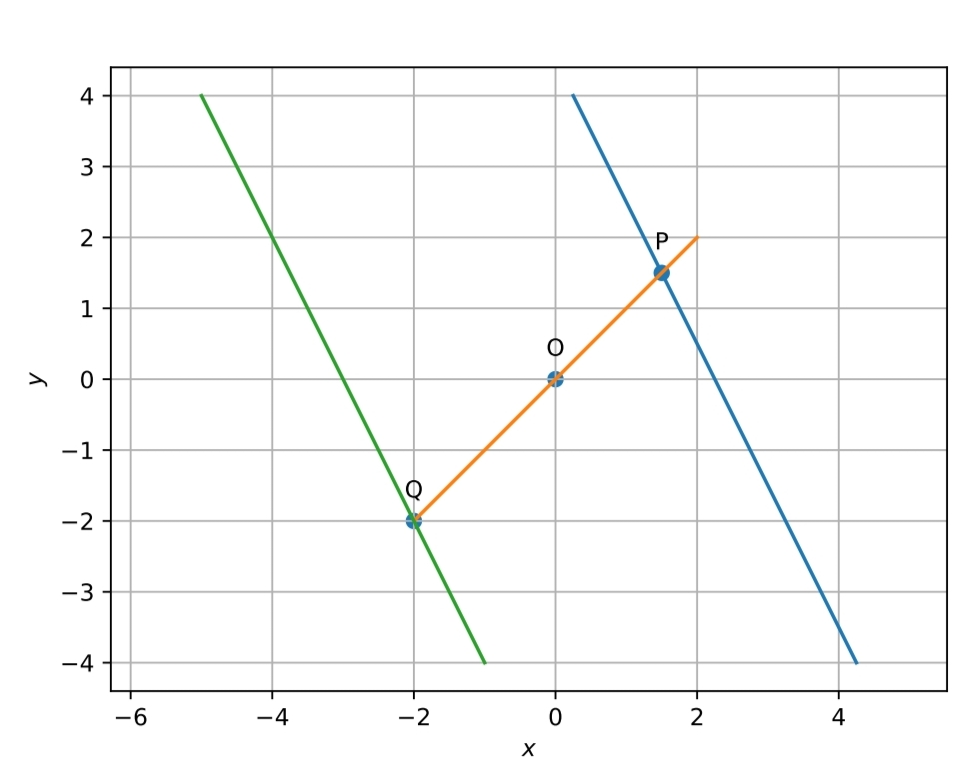
\includegraphics[width=0.5\textwidth]{line.jpg}  
\end{center}
\vspace{5mm}
 \vspace{2mm} 
\end{document}

